\documentclass{article}
\usepackage{ctex}
\usepackage{xcolor}
\usepackage[normalem]{ulem}
\usepackage[
colorlinks=true,
urlcolor=cyan,
linkcolor=cyan
]{hyperref}
\usepackage[a4paper,margin=1in]{geometry}
\usepackage{minted}
\usepackage{tikz}
\usepackage{graphicx}
\usetikzlibrary{positioning,arrows.meta,shapes.geometric}

\definecolor{codebg}{RGB}{230,230,230}
\setminted{
	breaklines=true,
	breakanywhere=true,
	bgcolor=codebg,
	fontsize=\small,
	linenos
}

\begin{document}

\section{目录}
\begin{enumerate}
	\item \hyperref[sec:developers]{开发者}
	\item \hyperref[sec:schedule]{开发日程}
	\item \hyperref[sec:system]{系统介绍}
	\item \hyperref[sec:instruction]{使用说明}
	\item \hyperref[sec:conclusion]{开源和AI使用以及思考总结}
\end{enumerate}

\section{开发者}
\label{sec:developers}
\begin{enumerate}
	\item 肖永恒：键盘输入、LED显示、数码管显示等硬件交互
	\item 邓科南：饮料列表模块和输入模式
	\item 高万里：顶层模块、总体逻辑以及引脚约束
\end{enumerate}


\section{开发日程}
\label{sec:schedule}

\begin{enumerate}
	
	\item github link: \href{https://github.com/Xiaomony/DigitLogicProject}
	{\uline{https://github.com/Xiaomony/DigitLogicProject}}
	
	\item 项目日程安排：
	\begin{enumerate}
		\item 第10周：项目讨论及整体设计
		\item 第11-13周：项目开发
		\item 第14周：整体测试
	\end{enumerate}
	
	\item 版本修改记录：
	
	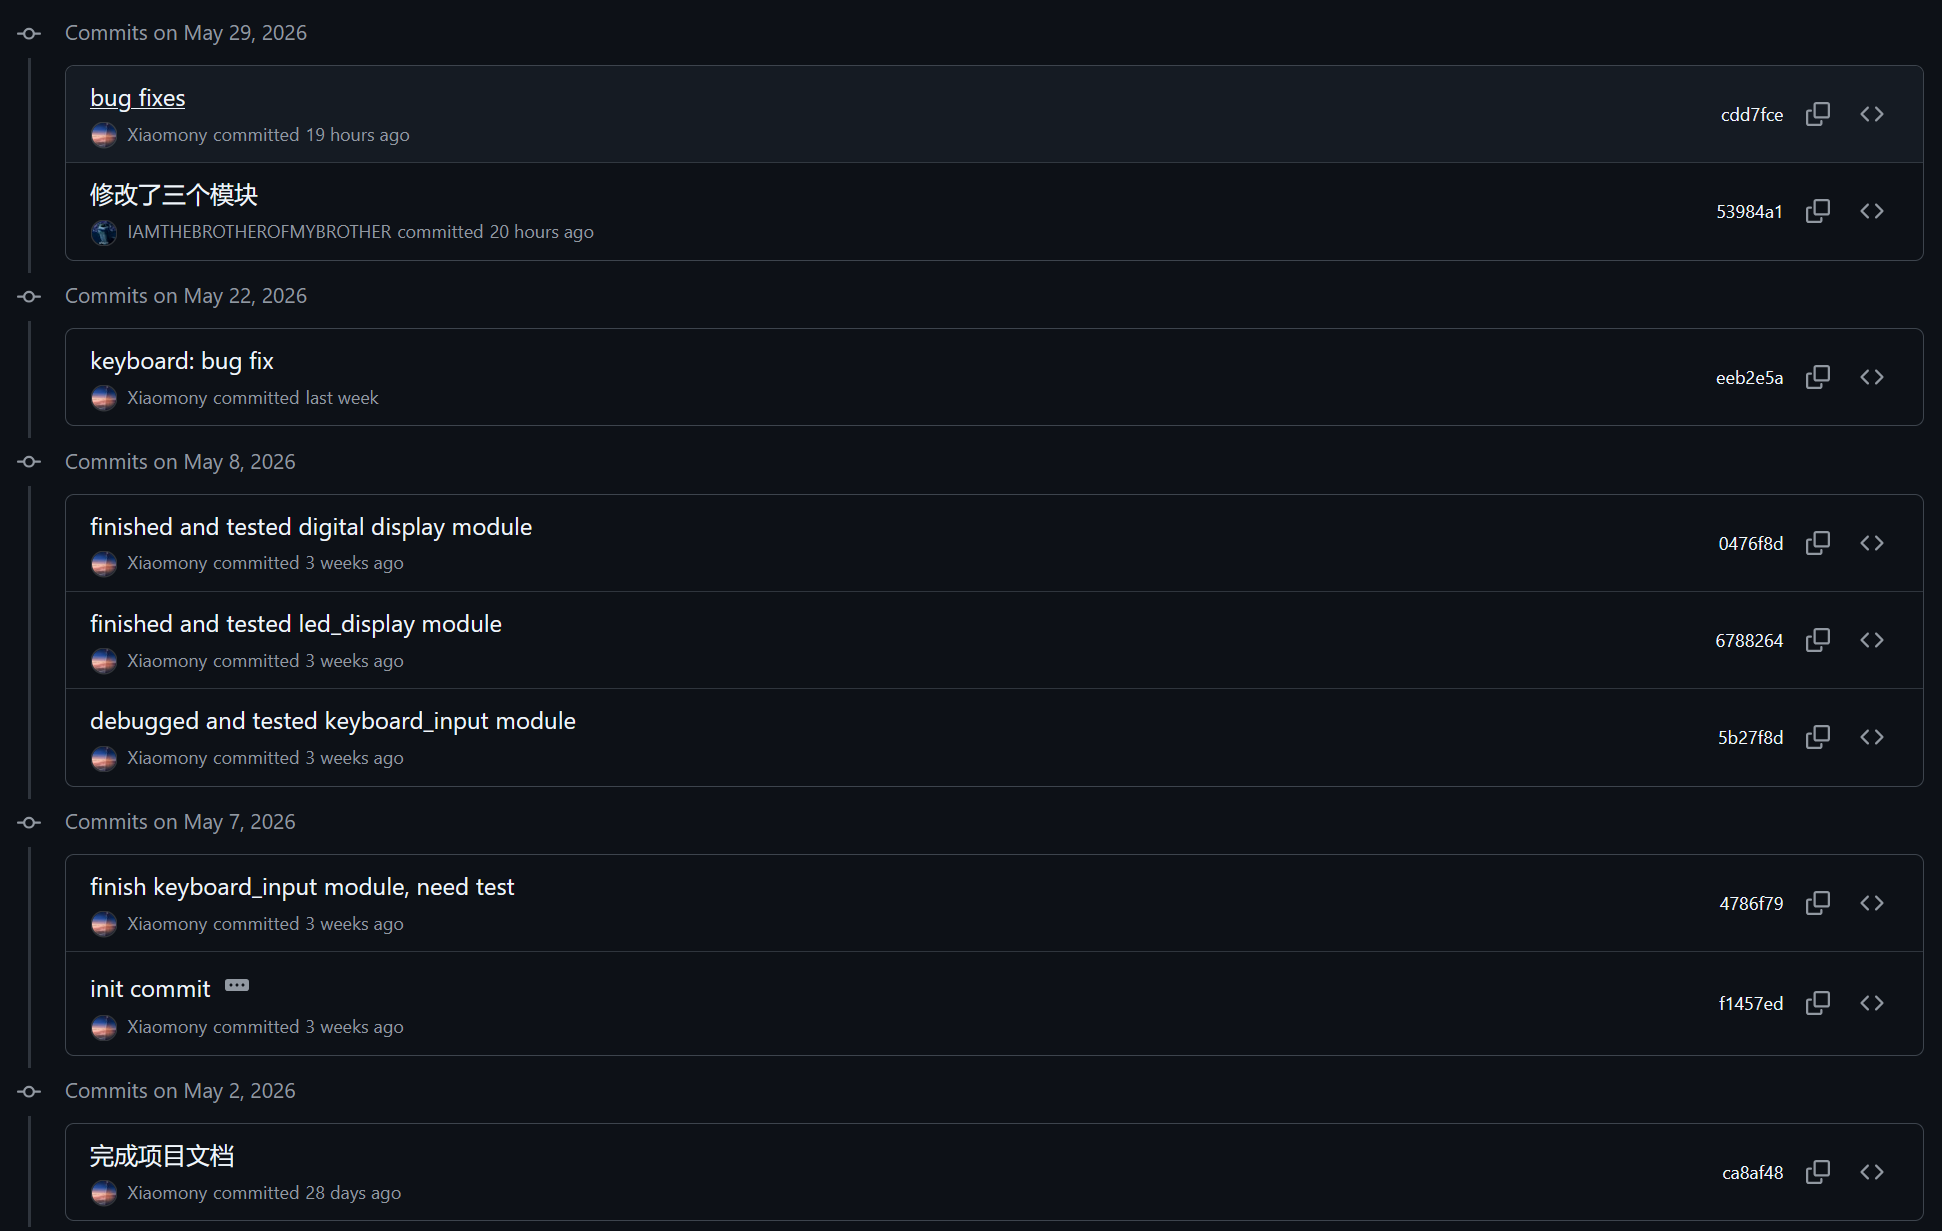
\includegraphics[width=0.99\textwidth]{res/git_commits.png}
	
\end{enumerate}


\newpage
\section{相关外设}
\subsection{键盘}
主要用到的按键，\textbf{\textit{详细用法见下方\hyperref[sec:states_diagram]{流程图}}}：
\begin{enumerate}
	\item 数字键\textbf{\textit{（主键盘、小键盘等效）}}
	\item Esc键：在任意模式中，按ESC可以退出到上一级
	\item 方向键
	\item Backspace键：在输入余额的时候，按下backspace可以删除上一个字符
	\item Enter键\textbf{\textit{（主键盘、小键盘等效）}}
\end{enumerate}

\subsection{8位数码管}
\begin{enumerate}
	\item 菜单状态：显示\textbf{\textit{\texttt{1SAL2SUP}}}，代表\textbf{\textit{1 Sale 2 Supervisor}}
	\item 饮料列表状态：8个数码管被分为两两一组，每次显示一个饮料，可用键盘上下键翻动或者数字键跳转到对应编号

		1--2为饮料编号；3--4为饮料的英文简写；5--6为饮料的单价；7--8为剩余库存，如果当前饮料为停售则显示两个下划线(\_\_)
\end{enumerate}

\subsection{LED}
\begin{enumerate}
	\item 最左侧LED亮起：当前处于销售模式
	\item 最右侧LED亮起：当前处于管理模式
	\item LED闪烁：报错
	\item 流水灯：处于菜单界面或者等待取货
\end{enumerate}

\section{系统介绍}
\label{sec:system}
\subsection{状态流程图}
\label{sec:states_diagram}
\subsubsection{主逻辑}
\begin{tikzpicture}[
	node distance=2cm,
	process/.style={
		align=center,
		rectangle,
		draw,
		rounded corners,
		minimum width=3cm,
		minimum height=1cm
	},
	small_process/.style={
		rectangle,
		draw,
		rounded corners,
		minimum width=1.5cm,
		minimum height=1cm
	},
	decision/.style={
		diamond,
		draw,
		aspect=2
	}
	]
	\node (menu) [process] {主菜单};
	
	
	% menu items
	\node (sale) [process, below left=0.5cm and 3cm of menu] {销售模式};
	\node (err) [process, below=1.5cm of menu] {报错状态\\LED闪烁,数码管显示错误码};
	\node (drink_list) [process, below=1.5cm of err] {饮料列表};
	\draw[->] (menu) -- node[midway, above]{数字键1} (sale);
	\draw[->] (sale) -- node[left]{无管理权限} (drink_list);
	
	% password check
	\node (pwd) [process, below right=0.5cm and 3cm of menu] {密码输入};
	\node (check) [decision, below=0.5cm of pwd] {密码正确?};
	\node (profit) [process, below=0.5cm of check] {显示盈利};
	\draw[->] (pwd) -- (check);
	\draw[->] (check) -- node[above]{否} (err);
	\draw[->] (check) -- node[left]{是} (profit);
	\draw[->] (profit) -- node[midway, above]{Enter} node[midway, below]{有管理权限} (drink_list);
	\draw[->] (menu) -- node[midway, above]{数字键2} (pwd);
	
	% manager mode
	\node (dl_admin) [process, below right=1.5cm and 2cm of drink_list] {管理模式(右LED亮)};
	\node (modify_inventory) [small_process, below left=1.5cm and 0.5cm of dl_admin] {修改库存};
	\node (modify_salable) [small_process, below=1.5cm of dl_admin] {翻转在售/停售};
	\node (modify_price) [small_process, below right=1.5cm and 0.5cm of dl_admin] {修改单价};
	\node (input_in_admin) [process, below=1cm of modify_salable] {输入模式};
	
	\node (success_in_admin) [small_process, below left = 1cm and 1mm of input_in_admin] {成功};
	\node (cancle_in_admin) [small_process, below right = 1cm and 1mm of input_in_admin] {取消};
	
	\draw[->] (drink_list) -- node[left]{有管理权限} (dl_admin);
	\draw[->] (dl_admin) -- node[left]{数字键1} (modify_inventory);
	\draw[->] (dl_admin) -- node[midway]{数字键2} (modify_salable);
	\draw[->] (dl_admin) -- node[right]{数字键3} (modify_price);
	
	\draw[->] (modify_inventory) -- (input_in_admin);
	\draw[->] (modify_price) -- (input_in_admin);
	
	\draw[->] (input_in_admin) -- node[left]{Enter} (success_in_admin);
	\draw[->] (input_in_admin) -- node[right]{Esc} (cancle_in_admin);
	
	% sale mode
	\node (dl_customer) [process, left=2cm of drink_list] {销售模式(左LED亮)};
	\node (input_in_customer) [process, below=1cm of dl_customer] {输入模式(输入余额)};
	\node (is_money_enough) [decision, below=0.5cm of input_in_customer] {余额充足?};
	\node (waiting_pick) [process, below=0.5cm of is_money_enough] {等待取货(流水灯)};
	\node (picked) [process, below=1cm of waiting_pick] {取货成功(显示余额)};
	\node (return_cargo) [process, below right=1cm and 0.5cm of waiting_pick] {退货};
	
	\draw[->] (drink_list) -- node[below]{无管理权限} (dl_customer);
	\draw[->] (dl_customer) -- node[right]{Enter} (input_in_customer);
	\draw[->] (input_in_customer) -- (is_money_enough);
	\draw[->] (is_money_enough) to[bend right=50] node[right]{否} (err);
	\draw[->] (is_money_enough) -- node[right]{是} (waiting_pick);
	\draw[->] (waiting_pick) -- node[right]{Enter} (picked);
	\draw[->] (waiting_pick) -- node[right]{5秒未取} (return_cargo);
	
\end{tikzpicture}

\subsubsection{输入模式}
\begin{tikzpicture}[
	>=Stealth,
	node distance=2cm,
	state/.style={
		rectangle,
		rounded corners,
		draw,
		align=center,
		minimum width=3cm,
		minimum height=1cm
	}
	]
	
	\node[state] (input) {输入模式};
	\node[state] (append) [left=of input] {追加到末尾};
	\node[state] (backspace) [right=of input] {删除末尾};
	\node[state] (confirm) [below left=1cm and 0cm of input] {确认};
	\node[state] (cancel) [below right=1cm and 0cm of input] {取消};
	
	\draw[->] (input) -- node[midway,above]{数字键} (append);
	\draw[->] (append) -- (input);
	\draw[->] (input) -- node[midway,above]{Backspace} (backspace);
	\draw[->] (backspace) -- (input);
	\draw[->] (input) -- node[midway,left]{Enter} (confirm);
	\draw[->] (input) -- node[midway,right]{Esc} (cancel);
	
\end{tikzpicture}

\subsubsection{饮料列表操作}
\begin{tikzpicture}[
	>=Stealth,
	node distance=2cm,
	state/.style={
		rectangle,
		rounded corners,
		draw,
		align=center,
		minimum width=4cm,
		minimum height=1cm
	}
	]
	
	\node[state] (list) {饮料列表\\显示当前饮料};
	\node[state] (up) [left=1cm of list] {显示上一种饮料};
	\node[state] (down) [right=1cm of list] {显示下一种饮料};
	\node[state] (jump) [below=1cm of list] {跳转到目标饮料};
	
	\draw[->] (list) -- node[midway,above]{↑} (up);
	\draw[->] (list) -- node[midway,above]{↓} (down);
	\draw[->] (list) -- node[midway,right]{数字键} (jump);
\end{tikzpicture}

\subsection{错误码}
\begin{enumerate}
	\item \texttt{NO PIC}：5秒内未取货
	\item \texttt{Err PAY}：余额不足
	\item \texttt{Err Stoc}：Stock，选择的饮料缺货
	\item \texttt{Err OFSA}：OFF SALE，选择的饮料已停售
	
\end{enumerate}

\subsection{系统架构及模块接口}
模块：
\begin{enumerate}
	\item \texttt{top}：顶层模块，负责组织所有子模块，{\Large\textbf{\textit{以下所有模块都直接隶属于顶层}}}
	
	\item 输入输出与硬件交互模块
	\begin{enumerate}
	
		\item \texttt{keyboard\_input}：负责处理键盘输入，\texttt{ps2\_clk}和\texttt{ps2\_data}分别绑定FPGA的K5、L4引脚，当读取到有效的按键的时候，\texttt{signal}将在接下来的一个时钟周期被变为1，且\texttt{keycode}变为读取到的按键的自定义键码
			\begin{minted}{verilog}
module keyboard_input(input clk, input ps2_clk, input ps2_data, output signal, output [3:0]keycode);
			\end{minted}
			
		\item \texttt{digital\_display}：负责数码管显示，\texttt{digit0}到\texttt{digit7}为从右到左8个数码管要显示的数字的段信号，\texttt{seg0}对应FPGA的左侧4个数码管的段信号，\texttt{seg1}对应FPGA的右侧4个数码管的段信号，\texttt{fragment}对应片选信号
			\begin{minted}{verilog}
module digital_display(input clk,
	input [7:0]digit0, input [7:0]digit1, input [7:0]digit2, input [7:0]digit3,
	input [7:0]digit4, input [7:0]digit5, input [7:0]digit6, input [7:0]digit7,
	output [7:0]seg0, output [7:0]seg1, output [7:0]fragment);
			\end{minted}
		
		\item \texttt{led\_display}：负责控制LED，\texttt{led\_out}对应从左到右8个大LED的引脚，\texttt{state}为LED状态
		\begin{minted}{verilog}
module led_display(input clk, input [1:0]state, output [7:0]led_out);
		\end{minted}
	\end{enumerate}
	
	\item 主要逻辑模块
	\begin{enumerate}
		\item \texttt{drink\_list}：饮料列表模块
			
			\texttt{manager} 为 1 时拥有管理权限
			
			\texttt{operation} 为当前需要执行的操作，所有操作均应只持续一个时钟周期，随后恢复为 \texttt{OP\_NONE}
			
			\texttt{op\_detail} 为 7 bit 数据（取值范围 0--127），其含义取决于当前操作：
			\begin{enumerate}
				\item 当修改库存时，\texttt{op\_detail} 表示新的库存数量；
				\item 当修改单价时，\texttt{op\_detail} 表示新的商品单价；
				\item 当执行跳转操作时，\texttt{op\_detail} 表示目标饮料编号；
				\item 当确认购买时，\texttt{op\_detail} 表示用户当前余额；
				\item 其余操作下忽略该参数。
			\end{enumerate}
			
			\texttt{profit} 为总销售额（13 bit，取值范围 0--8191）。
			
			\texttt{warning} 为报错信号。当发生错误时，该信号在一个时钟周期内被置为 1，随后自动恢复为 0
			
			\texttt{digit0} $\sim$ \texttt{digit7} 为当前 8 个数码管应显示的段选信号
			
			\begin{minted}{verilog}
module drink_list(input clk, input manager,
	input [2:0] operation, input [6:0]op_detail,
	output [12:0]profit, output warning,
	output [7:0]digit0, output [7:0]digit1,
	output [7:0]digit2, output [7:0]digit3,
	output [7:0]digit4, output [7:0]digit5,
	output [7:0]digit6, output [7:0]digit7);
			\end{minted}
		
		
		\item \texttt{input\_mode}：输入模式，\texttt{operation}为需要进行的操作，\texttt{digit0} $\sim$ \texttt{digit7} 为输入模式时从右到左8个数码管需要显示的段信号
			\begin{minted}{verilog}
module input_mode(input clk, input [3:0] operation,
	output [7:0]digit0, output [7:0]digit1,
	output [7:0]digit2, output [7:0]digit3,
	output [7:0]digit4, output [7:0]digit5,
	output [7:0]digit6, output [7:0]digit7);
			\end{minted}
		
		\item \texttt{devide\_frequency}：分频器
			\begin{minted}{verilog}
module devide_frequency #(parameter PERIOD=250_000)(input clk, output tick);
			\end{minted}
	\end{enumerate}
\end{enumerate}

\section{使用说明}
\label{sec:instruction}
\subsection{测试1}
	进入菜单后，按下1进入销售模式，使用上下按键翻动列表，或者使用数字键跳转到相应编号的饮料

	选择好饮料后，按下Enter键，输入不足的余额，再次按下Enter键，由于余额不足会进入报错状态，LED闪烁
	
	按下Esc退出销售模式，回到菜单，按下2键进入管理模式
	
	此时会要求输入密码，密码为12345678，输入后按下Enter进入管理模式，选择刚刚需要购买的饮料，按下3键修改其单价
	
	回到销售模式后，刚刚的饮料单价降低，选择好饮料后，按下Enter键，输入足够的余额，再次按下Enter键，LED会进入流水灯状态，等待取货，此时按下Enter键取货成功，可以看到饮料列表中显示的剩余库存减少了一个
\subsection{测试2}
	进入菜单后，按下2进入管理模式，使用上下按键翻动列表，选择一个饮料
	
	选择好饮料后，按下2键，将其转化为停售，再选择另一个饮料，按下1键，修改其库存为0、
	
	按Esc回到菜单，按下1键，选择停售的饮料，按下Enter购买，此时会报错，LED闪烁并且数码管显示错误码
	
	选择库存为0的饮料，按下Enter购买，此时会报错，LED闪烁并且数码管显示错误码
	
	选择一个有货的饮料，按下Enter并输入充足余额，LED会进入流水灯状态，等待取货
	
	此时等待5秒不取货，可以看到LED闪烁并退货，数码管显示\texttt{NO PIC}，库存未发生变化
	
\section{开源和AI使用以及思考总结}
\label{sec:conclusion}
\subsection{AI声明}
本项目中有关键盘PS2端口协议、跨时钟域信号同步的技术参考了AI给出的信息，本项目无通过vibe coding直接生成的代码。

项目文档部分使用AI生成且均经人工审查。
\subsection{项目总结}
本次数字逻辑课程设计以 FPGA 自动售货机为主题，综合运用了 Verilog HDL、状态机设计、模块化设计以及 FPGA 外设驱动等知识，实现了键盘输入、数码管显示、LED 状态指示、商品管理与销售等功能。通过本项目，我们对数字系统从需求分析、模块划分、接口设计到最终硬件验证的完整开发流程有了更加深入的理解。

在项目实现过程中，我们首先对整体功能进行了状态机建模，将系统划分为主菜单、销售模式、管理模式、输入模式、报错状态以及取货状态等多个状态，并进一步拆分为键盘输入、饮料列表管理、输入处理、LED 显示和数码管驱动等独立模块。通过明确各模块的职责和接口，降低了系统复杂度，提高了代码的可维护性和可扩展性。

开发过程中也遇到了许多实际问题。例如，在 PS/2 键盘驱动调试阶段，仿真结果正常但实际烧录后无法正确识别按键。经过分析发现，PS/2 信号属于异步输入，需要进行同步处理以避免亚稳态问题。同时，由于开发板内部 USB 转 PS/2 转换器输出的是 Scan Code Set 3，而非最常见的 Set 2，因此需要重新测量并整理对应的扫描码表。通过逻辑分析和硬件测试，最终解决了按键识别异常的问题。这一过程使我们认识到仿真与实际硬件运行环境之间存在差异，硬件调试能力同样是 FPGA 开发的重要组成部分。

此外，在数码管显示、LED 动画效果以及状态切换逻辑设计过程中，我们进一步熟悉了时序逻辑设计方法，理解了阻塞赋值与非阻塞赋值的区别，以及同步时钟设计的重要性。通过不断测试和修改，最终实现了预期功能。

\end{document}
